\chapter{Introduction}
\titlespacing*{\chapter}{0pt}{-50pt}{40pt}
\label{Chapter1} % For referencing the chapter elsewhere, use \ref{Chapter1} 

\lhead{Chapter 1. \emph{Chapter Title Here}} % This is for the header on each page - perhaps a shortened title

%----------------------------------------------------------------------------------------
\begin{quotation}
Underwater Sensor Networks (UWSNs) provide an enabling technology for the development of ocean observation systems. Application domains of UWSNs include military surveillance, disaster prevention, assisted navigation, offshore exploration, tsunami monitoring, oceanographic data collection, to mention a few. Many of the above mentioned applications utilize UWSNs nodes that may move freely with water currents. Thus, node locations at any instant can only be specified probabilistically. When connectivity among some of the sensor nodes is required to perform a given function, the problem of estimating the likelihood that the network achieves such connectivity arises.

In this chapter, we give an overview of UWSNs, highlight some research work done in the area, and discuss some related node mobility  models used by networking researchers in the area. Next, we introduce a probabilistic mobility model that is used to formalize the problems considered in the thesis. We conclude by outlining thesis contributions.
 \end{quotation}
\section{Introduction}
\label{ch1:intro}
In recent years, underwater sensor networks (UWSNs) have attracted considerable attention in networking research.
A typical UWSN is conceived to have a number of sensor nodes that can perform sensing tasks, data storage and processing tasks, and data communication tasks.
Drifters and RAFOS floats (see, e.g., \cite{bower1989evidence}) are examples of devices with no self-controlled mobility that have been used in real oceanography experiments. In addition to such devices, modern UWSNs utilize Autonomous Underwater Vehicles (AUVs) with self-controlled mobility.
Several surveys on the history, architecture, potential applications, and design and implementation challenges of UWSNs appear in \cite{akyildiz2005underwater, partan2007survey, heidemann2012underwater, climent2014underwater, gkikopouli2012survey}.
In this introduction, we highlight some of these aspects to motivate the particular research direction taken in the thesis.



To start, we mention that interest in UWSNs research has been fuelled by many important underwater sensing applications and services that can be supported by such networks.
In  \cite{akyildiz2005underwater} and \cite{heidemann2012underwater}, for example, the domains of applications are classified as follows.
\begin{itemize}
\item \textbf{Scientific applications}: e.g., observing  geological processes on the ocean floor, determining water characteristics (e.g., temperature, salinity, oxygen levels, bacterial and other pollutant content, and dissolved matter), counting or imaging animal life (e.g., micro-organisms, fish or mammals, and coral reef)
\item \textbf{Industrial applications}: e.g., monitoring and control of commercial activities, determining routes for underwater cables, monitoring underwater equipment  and pipelines for oil and mineral extraction, and monitoring commercial fisheries
\item \textbf{Military and homeland security applications}: e.g., monitoring and securing port facilities

\item \textbf{Humanitarian applications}: e.g., search and survey missions, disaster prevention tasks (e.g., tsunami warning to coastal area), identification of seabed hazards, locating dangerous rocks or shoals, and identifying possible mooring locations
\end{itemize}

UWSNs are expected to provide better services in each of the above domains over the traditional approach of deploying underwater sensor devices that record data during a monitoring mission, and then recovering the devices at the end of a mission.
In \cite{akyildiz2005underwater}, the authors point out that compared to this traditional approach, UWSNs provide the following advantages:
\begin{itemize}[noitemsep]
\item supporting real time monitoring, since the observed data can be transmitted shortly after collection,
\item supporting better interaction between onshore control systems and the monitoring devices, and
\item supporting better handling of device failures and misconfigurations.
\end{itemize}
It has also been emphasized in the above survey papers that UWSNs are expected to be sparser than terrestrial wireless sensor networks (WSNs) since individual nodes in UWSNs have significantly more cost compared to nodes in terrestrial WSNs. In addition, many UWSNs are required to cover relatively larger water areas.

The design and implementation of cost effective UWSNs to serve the above applications, however, face a number of challenges.
Some of these challenges are attributed to the current technological limitations of dealing with the underwater communication channel. Other challenges are attributed to the harsh environment of underwater environments.

\textbf{Challenges of the underwater communication channel.} Unlike terrestrial-based WSNs that enjoy low delay and high bandwidth networking devices, UWSNs face significant challenges in getting adequate communication bandwidth.  To see this, we summarize below some of the findings emphasized in \cite{partan2007survey} and  \cite{akyildiz2005underwater} on the use of radio frequency communication, optical communication, and acoustic communication for UWSNs. (All frequencies, bandwidths, distances, and data rates given below are approximate values or ranges to illustrate the main findings.)



\begin{itemize}
\item \textbf{Radio frequency communication.} The majority of radio frequencies suffer strong attenuation in salt water. Long-wave radio (1-100 KHz) can be used for short distances (6-20 m) and low data rates (1 Kbps). Communication with long-wave radio, however, requires large antennas and high transmission power.
In the past, communication to a satellite has been used to send the collected data when an UWSN node floats on water surface after completing a mission.

\item \textbf{Optical communication.} Light is also strongly scattered and absorbed underwater. In \cite{partan2007survey}, it is pointed out that blue-green wavelengths may be used for short-range, high bandwidth connections in extremely clear water.
Thus, optical communication in UWSNs are limited to short distances ($\leq 40$ m) using directed transmission over unobstructed line-of-sight communication.
Low cost optical communication for very short connections (1-2 m) at rates of 57 Kbps has been considered in \cite{fair2006optical, freitag2001acoustic}.

\item \textbf{Acoustic communication.} Sound also suffers from various factors of attenuation, spreading, as well as man-made noise, and ambient noise in underwater. 
Acoustic communication, however, is currently perceived as the most practical method.
In \cite{akyildiz2005underwater}, the authors take a closer look at the capabilities of current acoustic modems. 
They classify the available bandwidth for different distance ranges in UW acoustic channel as follows (for brevity, we use the notation [\textbf{distance range, bandwidth}] to present the classification):  very long [1000 Km, $<$ 1 KHz], long [10-100 Km, 2-5 KHz], medium [1-10 Km, $\approx$ 10 KHz], short [0.1-1 Km, 20-50 KHz], and very short [$<$ 0.1 Km, $>$ 100 KHz].
The speed of sound underwater is approximately 1500 m$/$s, which is $2\times 10^5$ times lower than the speed of light. 
So, acoustic communication suffers from long delays as well.
Standard acoustic transducers can be relatively big in size, heavy weight, and power hungry. In \cite{partan2007survey}, the authors point out that on compact stationary sensor nodes, and space-constraint AUVs, transducers generally cannot be spatially separated far enough to provide full-duplex connections since the transmitted signals will saturate the receiver even when the communication bands are fairly widely separated.
Thus, underwater networks are expected to utilize half-duplex connections.
\end{itemize}

The above challenges in supporting low delay and high data rate communication have triggered research work in almost all areas of the UW networking protocol stack.
The following surveys are particular to UWSNs: Medium Access Control (MAC) protocols \cite{Farrell2012, yunus2010survey, petrioli2008comparative, yigitel2011qos, chen2014}, routing  \cite{ayaz2011survey, pompili2006routing, bayrakdar2011comparative, giantsis2011comparison}, localization \cite{chandrasekhar2006localization, zhou2010efficient, zhou2011scalable, tan2011survey, erol2011performance}, connectivity and coverage \cite{ghosh2008coverage, zhu2012survey}.  Examples of research work done on connectivity, coverage, and deployments appear in \cite{senel2013autonomous, akkaya2009self, ammari2010study, Nazrul2008,  reza2009robust}.


\textbf{Challenges due to node mobility.} To serve the diverse types of applications mentioned above, various types of UWSN deployments are used.
In \cite{heidemann2012underwater}, for example (see, e.g., figure \ref{fig:Exm111}), UWSN deployments are
classified as being either static, semi-mobile, or mobile.
%
Static networks have nodes attached to underwater ground,
anchored buoys, or docks.
%
Semi-mobile networks may have collection of nodes attached to a
free floating buoy. Nodes in semi-mobile networks are subject to small scale
movements.
%
Mobile networks may be composed of drifters with no self mobility
capability, or nodes with mobility capability. Nodes in such networks
are subject to large scale movements.
%
UWSN deployments may occur over many short periods of times (e.g.,
several days at a time), so as to conduct several missions over
a large area of interest.
\begin{figure}[h]
\centering
\includegraphics[width=5 in, height=2.5 in]{UnderwaterScnerio1.pdf}
 \caption{ Example UWSNs.}
 \label{fig:Exm111}
\end{figure}
Maintaining connectivity in such networks is a crucial aspect for performing many tasks that require node collaboration.
Examples of such tasks include localization \cite{teymorian20093d, erol2008multi, isik2009three, zhou2010efficient, zhou2011scalable, erol2011performance}, routing \cite{noh2013vapr, ying2011combining, lee2010pressure, ren2012performance} and coverage \cite{ammari2010study, senel2013autonomous, akkaya2009self, pompili2006deployment}.

In this thesis, we consider semi-mobile and mobile networks.
Our interest is in developing methodologies that allow a designer to analyze the likelihood that a network (or part of it) is connected at a given time interval.
In the next section, we review some work on quantifying node mobility models used by networking researchers for UWSNs.

\section{Node Mobility}
\label{ch1:wounmm}

One may classify node mobility in UWSNs into controllable mobility (C-mobility for short), and uncontrollable mobility (U-mobility).
The simplest type of C-mobility is vertical movements induced by mechanical devices inside a node \cite{erol2008multi, Erol:2007}.
Full 3D C-mobility is enjoyed by AUVs at the expense of node energy consumption.
U-mobility, on the other hand, is primarily due to surface and subsurface water currents, as well as wind.
Findings of real ocean measurements, as well as a large body of analytical results in oceanography have shaped the understanding of networking researchers in this area.


We note that this area is new to networking researchers where the obtained analytical results are rooted in the mathematically deep field of fluid dynamics.
The thesis work makes an effort to summarize some of the important findings in this regard.
Our goal in this section is to foster the idea that numerical values for the probabilistic locality model used throughout the thesis can be deduced from the available empirical measurements of node mobility, and the obtained analytical models that capture the behaviour found in the empirical results.


The probabilistic node locality adopted in the thesis divides the geographic area containing nodes into rectangles of an (imaginary) superimposed grid layout.
After a given time period following network deployment in water, each node $x$ can be in any one of a possible set of grid rectangles, denoted $Loc(x) = \{x[1], x[2],\ldots\}$.
We call $Loc(x)$ the locality set of $x$. 
Thus, depending on the mobility model induced by water currents, node $x$ can be in any possible grid rectangle $x[i]\in Loc(x)$ with a certain probability, denoted $p_x(i)$.


To explain that such probability distribution can be deduced from empirical experiments, we refer to the important work of \cite{bower1989evidence} which has triggered intensive work in the area.
In \cite{bower1989evidence}, the authors report on several observations collected in the Gulf Stream using thirty-seven RAFOS drifters launched off Cape Hatteras.
Mobility of the free floating drifters is tracked for 30 or 45 days.
Among the collected observations, the authors determined the geographic location of each of the 37 drifters at each day of the observation period.
Given the exact geographic location of each drifter in each day, one can superimpose a virtual grid (of some user specified dimensions per rectangle) on the area traversed by the floats and use the reported locations to derive rough values of the probabilities used in our probabilistic locality model.


Next, we present our findings on the use of the available analytical mobility models to derive the probabilities used in our model.
In \cite{bower1989evidence}, the authors observed striking patterns of cross-stream and vertical motion associated with meanders in the Gulf Stream.
Later, in \cite{bower1991simple}, the author introduced a 2D kinematic model that captures many of the important patterns observed in \cite{bower1989evidence} including the effect of meandering sub-surface currents and vortices on free floating drifters.
The introduction of such kinematic model has resulted in a large body of subsequent analytical work in the area.
Recently, this kinematic model has received attention in networking literature.
Following a similar approach, \cite{caruso2008meandering} devised a kinematic mobility model for UWSNs, called the meandering current mobility model.
The model is useful for large coastal environments that span several kilometres.
It captures the strong correlations in mobility of nearby sensor nodes.
In \cite{caruso2008meandering}, the model has been used to analyze several network connectivity, coverage, and localization aspects of UWSNs by simulation.

\textbf{The kinematic model of \cite{caruso2008meandering}}. To explain the model presented in \cite{caruso2008meandering}, we start by recalling some concepts from fluid dynamics (see, e.g., \cite{yunus2013fluid}).
A particle \textit{pathline} is a path followed by an individual particle in a flow.
A \textit{stream} function is a scalar function, denoted  $\psi$, that measures the volume flow rate per unit depth at a point with coordinate $(x,y)$.
Curves where $\psi$ is constant are called \textit{streamlines}.
For steady flows, streamlines and particle paths coincide.
In 2D, a stream function has the property that the $x$ and $y$ velocity vectors ($\dot{x}$ and $\dot{y}$ ) can be obtained by taking partial derivatives of the stream function, as shown below.
The stream function adopted in \cite{caruso2008meandering} utilizes also time (the parameter $t$) to determine the function value, as follows:

\begin{equation}\label{eq:sf}
\psi(x,y,t)=-\tanh{[\frac{y-B(t)\sin(k(x-ct))}{\sqrt{1 + k^2 B^2(t) \cos^2(k(x-ct))}} ]} + cy
\end{equation}
 where $  B(t) = A + \epsilon \cos(\omega t)$  and the $x$ and $y$ velocities are given by
 
 \begin{equation}\label{eq:lf}
\dot{x}=-\frac{\partial \psi}{\partial y} ; \dot{y}=\frac{\partial \psi}{\partial x}
\end{equation}


The trajectory of a node that moves within the current is the solution of the above ordinary differential equations.
We now present the following remarks using the same parameter setting used in \cite{caruso2008meandering}. Namely, $A=1.2, c=0.12, k=\frac{2\pi}{7.5}, \omega=0.4$ and $\epsilon=0.3$, 

\begin{enumerate}
\item For a fixed $t$ (we use $t=0$), a plot of the stream function $\psi$ in $3D$ is shown in figure \ref{fig:kme3d}.
The plot shows that particles deployed at coordinates $x=0$ and $y\in [-2,+2]$ tend to follow sinusoidal pathlines, whereas particles deployed elsewhere may fall into circulations.
\begin{figure}[!htb]
\centering
\includegraphics[width=5 in, height=3 in]{BBC.pdf}
 \caption{ A 3D plot of stream function \ref{eq:sf}}
 \label{fig:kme3d}
\end{figure}

Figure \ref{fig:kme} illustrates the contours of the 3D plots when drawn in 2D.

\item We observe from figure \ref{fig:kme} that any particle deployed in the area shown stays within a strip of vertical height (along the $y$-axis) of $\pm$ 4 Kms.

\begin{figure}[!htb]
\centering
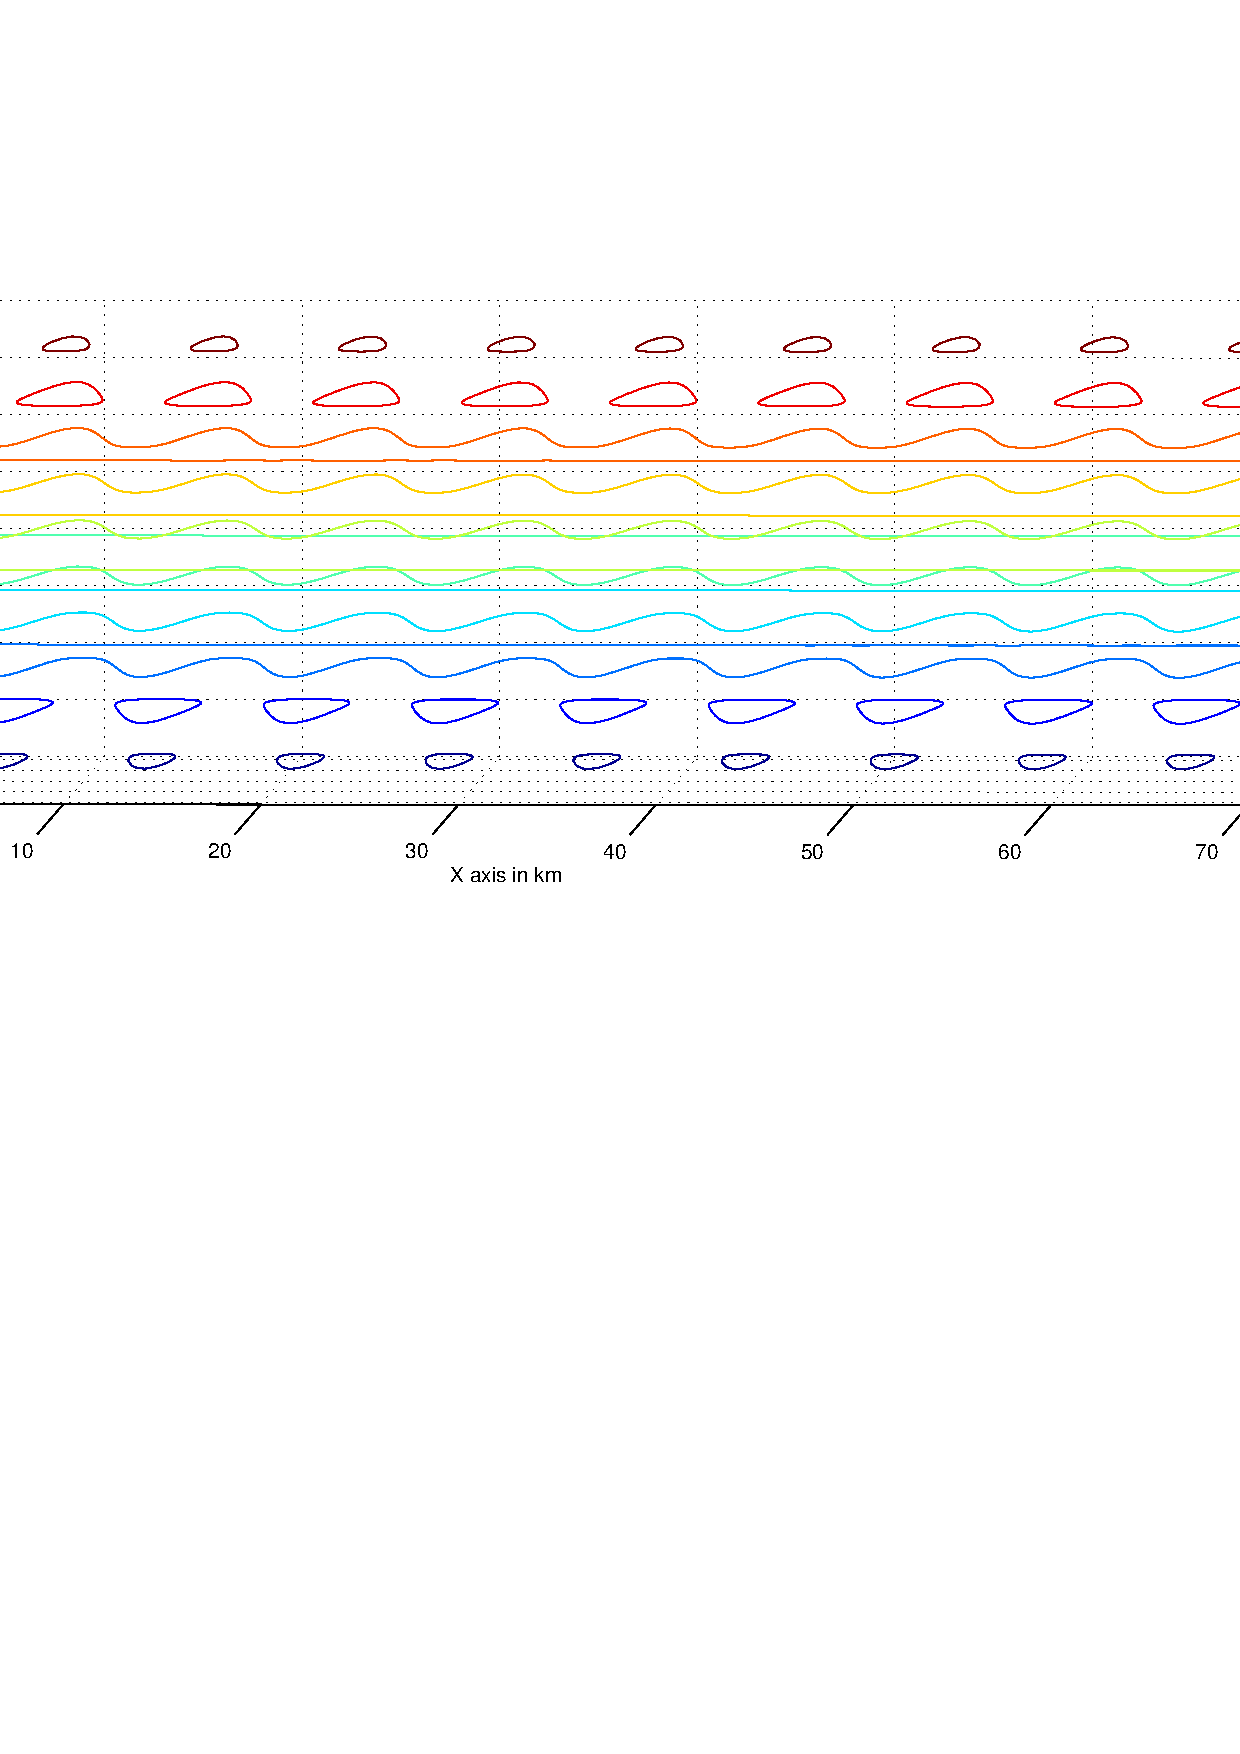
\includegraphics[width=5 in, height=2.5 in]{MCM.pdf}
 \caption{ A plot of stream function \ref{eq:sf} at $t=0$.}
 \label{fig:kme}
\end{figure}

\item Although the above ordinary differential equations are deterministic, small variations in the initial position of a node deployed at t=0 has a strong influence on the trajectory taken by the node (e.g., which circulations it falls into, and for how long).
Figure \ref{fig:res11} illustrates the findings of an experiment where a sample set of 50 nodes are deployed at $t= 0$ in a rectangle of narrow horizontal width at $x=0$, and vertical height in the range $y \in [1.00, 1.30]$ (300 meters). The trajectories are simulated for 2 days. The figure shows the initial positions of the 50 nodes on the left, and the end points of the trajectories at the end of the 2-day period. 
\begin{figure}[!htb]
\begin{minipage}[]{.55\linewidth}
\includegraphics[width=3 in, height=1.8 in]{Endpoints100.pdf}
 \caption{ Start and end points of 50 nodes}
\label{fig:res11}
\end{minipage}
\begin{minipage}{.45\linewidth}
\includegraphics[width=1.8 in, height=2 in,angle=-90]{Endpt.pdf}
 \caption{Probabilistic distribution obtained using a superimposed grid}
\label{fig:ges11}
 \end{minipage}
\end{figure}
\item The above type of simulation experiments can be used to derive the needed probabilities in our probabilistic locality model. For example, as done in figure \ref{fig:ges11}, one can superimpose a grid over the area encapsulating the end points of the 50 trajectories (i.e., the rectangle where $x \in$ [14 Km, 30 Km], and $y \in$ [$-3$ Km, $+2.2$ km]), we then can derive the probability that a node lands in a particular rectangle, say $R$, by dividing the number of end points landed in $R$ over the sample size (50 in this case).
\end{enumerate}
%------------------------------------


%In the next sections we outline the network model and problem formulations.

\section{Network Model}
\label{sec:Nmpf}
In this section, we introduce the concept of \textit{probabilistic graphs} used throughout the thesis. This concept is used to capture node location uncertainty common to UWSNs.

\subsection{Node Locality Sets}
\label{ch1:nls}
We consider UWSNs utilizing both sensor nodes and relay nodes. Sensor nodes can perform sensing, data storage, processing, and communication tasks. Relay nodes can perform data storage and communication only. Several studies on various types of networks have shown that relay nodes can save energy and enhance overall network performance.
We denote by $V=V_{sense}\cup V_{relay}$ the set of nodes in a given UWSN where $V_{sense}$ denotes sensor nodes, and $V_{relay}$ denotes relay nodes.
%
We assume that $V_{sense}$ has a distinguished {\em sink} node,
denoted $s$, that performs network wide command and control functions.


After some time interval $T$ from network deployment time,
each node $x$ can be in some location determined by water currents
causing node movement.


To simplify analysis, current approaches in the literature typically divide
the geographic area containing nodes into rectangles of a superimposed
grid layout.
%
Thus, at time $T,$ each node $x$ can be in any one of a possible
set of grid rectangles denoted $\loc(x)= \{ x[1], x[2], \ldots \}$.
%
We call $\loc(x)$ the {\em locality} set of $x$ (for simplicity,
we omit the dependency on $T$ from the notation).
%
Depending on the mobility model induced by water currents, node $x$
can be in any possible grid rectangle $x[i]$ with a certain probability,
denoted $p_x(i)$. 
%

As mentioned in Section \ref{ch1:wounmm}, one may utilize the kinematic model adopted in \cite{caruso2008meandering} to compute such probabilities from a sufficiently large number of node trajectories simulated by the model.

Henceforth, we use $x[i]$ to refer to node $x$ at the $i^{th}$ location index.
%
For brevity, we also refer to $x[i]$ as the location of $x$
(rather than the grid rectangle containing $x$) at an instant of interest.
%
To gain efficiency in solving large problem instances with large locality
sets, it may be convenient to truncate some locality sets to include only
locations of high occurrence probability, and ignore the remaining locations.
%
In such cases, we get $\sum_{x[i] \in \loc(x)} p_x(i) \leq 1$, if $\loc(x)$
is truncated.

% -------------------------

\subsection{Node Reachability}

At any instant, node $x$ can reach node $y$ if the acoustic signal strength
from $x$ to $y$ (and vice versa) exceeds a certain threshold value.
%
In acoustic UWSN, direction of water currents play an important role
in signal delay (see, e.g., \cite{pu2013comparing}).
%
For simplicity, we assume that given the exact locations of $x$ and $y$, say $x$ at location $x[i]$ and $y$ at location $y[j]$, we can determine if $x$ and $y$ can reach each other, and if so, we
set the link indicator $E_G (x[i],y[j])= 1$.
%
Else, if no satisfactory communication can take place then
we set $E_G (x[i],y[j])= 0$.


Our general objective in this thesis is to develop effective methodologies
for computing lower bounds on the likelihood that the network is totally,
or partially, connected.
%
To this end, we adopt the following rule: we set $E_G(x[i],y[j])= 1$
if and only if the two nodes $x$ and $y$ can reach each other if
they are located anywhere in their respective rectangles $x[i]$ and $y[j]$.


The above rule implies that connectivity between $x$ and $y$ is ignored if 
they can reach each other at some (but not all) pairs of points in their
respective rectangles.
%
As can be seen, ignoring connectivity in such cases results
in computing lower bounds on the network connectivity, as required.
%
Thus we model an UWSN by a probabilistic graph $G=(V=V_{sense}\cup V_{relay},E_G,Loc,p)$.

\section{Problem Formulation}
\label{ch1:pf}
In this section we formulate four probabilistic connectivity problems that we investigate in the thesis. 


\begin{definition}[\textbf{the $A$-$CONN$ problem}]
\normalfont
Given a probabilistic network $G$ with no relay nodes, compute the probability $Conn(G)$ that the network is in a state where the sink node $s$ can reach all sensor nodes. $\blacksquare$
\end{definition}


\begin{definition}[\textbf{the $AR$-$CONN$ problem}]
\normalfont
Given a probabilistic network $G$ where $V_{relay}$ is possibly non-empty, compute the probability $Conn(G)$ that the network is in a state where the sink node $s$ can reach all sensor nodes. $\blacksquare$
\end{definition}


\begin{definition}[\textbf{the $S$-$CONN$ problem}]
Given a probabilistic network $G$ with no relay nodes, and a required number of sensor nodes $n_{req}\leq |V_{sense}|$, compute the probability $Conn(G,n_{req})$ that the network is in a state where the sink node $s$ can reach a subset of sensor nodes having at least $n_{req}$ sensor nodes. $\blacksquare$
\end{definition}


\begin{definition}[\textbf{the $SR$-$CONN$ problem}]

Given a probabilistic network $G$ where $V_{relay}$ is possibly non-empty, and a required number of sensor nodes $n_{req}\leq |V_{sense}|$, compute the probability $Conn(G,n_{req})$ that the network is in a state where the sink node $s$ can reach a subset of sensor nodes having at least $n_{req}$ sensor nodes. $\blacksquare$
\end{definition}

We note some of the above problems are special cases of other problems. Using the polynomial time reducibility relation \cite{cormen2001introduction} denoted $\leq_p$, one can state the following:
\begin{itemize}
\item $\ACONN \leq_p \ARCONN$ and $\SCONN \leq_p \SRCONN$ (since $V_{relay}$ can be an empty set)
\item $\ACONN \leq_p \SCONN$, since $n_{req}$ can be set to $|V_{sense}|$.
\end{itemize}

We next remark that the above problems share some basic aspects with the class of network reliability problems discussed in \cite{Co87}. In particular, all such problems are defined over some type of probabilistic graphs. For network reliability problems, a node or link can either be operating or failed with some known probability, whereas in our present context, a node can be in any one of a possible set of locations with known probability distribution.

Events of interest on such probabilistic graphs occur when the given network is in some particular network states. In our present context, a \textbf{network state} $S$ of $G$ arises when each node $x \in V$ is located at some specific location in its respective locality set $Loc(x)$.
Thus, if $V = \{v_1 , v_2 , . . . , v_n \}$ then a state $S$ of $G$ can be specified by $\{v_1[i_1], v_2[i_2], . . . , v_n[i_n]\}$ where each $v_\alpha[i_\alpha] \in Loc(v_{\alpha})$. Two states $S_1$ and $S_2$ are different if they differ in the location of at least one node. Assuming node locations are independent of each other, we have $Pr(S) =\prod_{v_{\alpha}\in V} p_{v_\alpha[i_\alpha]}$.

{\bf Note:} For a node $v_{\alpha}\in V$ and a possible index $i_\alpha$ in the locality set of $v_{\alpha}$, our use of the notation $v_{\alpha}[i_{\alpha}]$ is overloaded. In some sentences, $v_{\alpha}[i_{\alpha}]$ refers to a particular rectangle in $Loc(v_{\alpha})$. In other sentences, $v_{\alpha}[i_{\alpha}]$ refers to node $v_{\alpha}$ when it is in the location indexed by $i_{\alpha}$ in its locality set. 


In the $A$-$CONN$ and $AR$-$CONN$ problem, a state is \textbf{operating} if the
sink $s$ can reach all sensor nodes in $V_{sense}$ . Likewise, in
the $S$-$CONN$ and $SR$-$CONN$ problem, a state $S$ is \textbf{operating} if the sink node $s$ can reach a subset having at least $n_{req}$ sensor
nodes. Let $\textbf{S}$ be the set of all operating states $S$ of a
given problem. Then the required solution is given by
$\sum_{S\in \textbf{S}} Pr(S)$.

\begin{example}
\normalfont
Figure \ref{fig:Exmp1} illustrates a probabilistic graph on 4 nodes where $V=\{s,a,b,c\}$ and the locality set of each node has 2 locations. The network has $2^4$ states. For the $A$-$CONN$ problem, state $S_1= \{ s[2], a[2], b[2], c[2] \}$ is operating, and
     state $S_2= \{ s[1], a[1], b[1], c[2] \}$ is failed. $\blacksquare$
\end{example}
\begin{figure}[h]
\centering
\includegraphics[width=3.5 in, height=1.8 in]{Figure1.pdf}
 \caption{ An example probabilistic network}
 \label{fig:Exmp1}
\end{figure}

\textbf{The Underlying Graph of Probabilistic Network.} Given a probabilistic network $G=(V,E_G,Loc,p)$ the \textit{underlying graph} of $G$ is an undirected graph $\tilde{G}$ where

\begin{enumerate}[noitemsep]
\item $V(\tilde{G})=V$.
\item $E(\tilde{G})$ has an edge $e=(x,y)$ if for some positions $x[i]$ and $y[j]$ of nodes $x$ and $y$, respectively, we have $E_G(x[i],y[j])=1$.
\end{enumerate}


\begin{example}
\normalfont
The underlying graph of the probabilistic network in figure \ref{fig:Exmp1} is the cycle $(s,a,c,b)$. $\blacksquare$
\end{example}

Equivalently, we say that the probabilistic network $G$ has the topology of the graph $\tilde{G}$. Throughout the thesis, we use the same symbol $G$ to refer to both a probabilistic network and its underlying graph. Overloading the use of the symbol $G$ does not cause confusion since the exact meaning can be deduced by context.
\section{Thesis Organization and Contribution}
\label{sec:thc}

The main research direction undertaken in the thesis is to develop efficient algorithms for handling the defined probabilistic connectivity problems on networks whose underlying graphs have some useful structure. The availability of such algorithms can be used to derive lower bounds on the probabilistic connectivity of any given arbitrary probabilistic network. This approach relies on identifying subgraphs with the desired structure in the graph underlying a given probabilistic network then solving a problem of interest on the identified subgraph.
The thesis pursues this general approach on the well known classes of partial $k$-trees, explained in Chapter 2. The remaining part of the thesis is organized as follows.
\begin{enumerate}
\item Chapter 2 is dedicated to reviewing basic definitions, properties, and algorithmic aspects of $k$-trees and partial $k$-trees.

\item Chapter 3 presents the first contribution of the thesis: an efficient dynamic programming algorithm to solve the $\SRCONN$ problem on probabilistic networks whose underlying graphs are trees. The algorithm solves the more restricted $\ARCONN$ problem with little overhead compared to a dedicated algorithm to solve the $\ARCONN$ problem.
\item Chapter 4 presents a second contribution of the thesis: a dynamic programming algorithm to solve the $\ACONN$ problem on partial $k$-trees. The algorithm runs in polynomial time for any fixed $k$.
\item Chapter 5 considers UWSNs with relay nodes. The chapter presents a third contribution: two dynamic programming algorithms to solve the $\ARCONN$ and $\SRCONN$ problems on partial $k$-trees. The algorithm runs in polynomial time for any fixed $k$. 
\end{enumerate}
Finally Chapter 6 concludes with remarks and possible future research directions

\section{Concluding Remarks}
\label{sec:cg1sum}
In this chapter, we have introduced the notion of a probabilistic network that captures node location uncertainty commonly encountered in UWSNs. Using the notion of probabilistic networks, we have formalized 4 concrete probabilistic connectivity problems whose solution can significantly benefit the design of UWSNs utilizing relay nodes. In the next chapter, we introduce the class of partial $k$-tree that enable the computation of lower bounds on the probabilistic connectivity problems of interest.
